\chapter{Electromagnetic waves in periodic media}
\label{ch:Electromagnetic waves in periodic media}

This chapter focuses on basic concepts and principles related to electromagnetic fields and waves based on Maxwell's equations. More over, some emphasis will be taken on stating these equations as a linear Hermitian Eigenvalue problem that has many common points with the Schr\"odinger equation and its application to crystals in the field of Solid State Physics \cite{Kittel2005}. 
In this way, propagation of light in a PC can be defined using linear operators acting over wave functions that are solution to a given eigenvalue problem.  Periodicity is then invoked by means of discrete translational symmetry operators, and their associated phase shift eigenvalue. 

\section{Maxwell equations}

The macroscopic behavior of electromagnetism, including propagation of light in Photonic Crystals (PCs) are governed by \textbf{Maxwell equations}. Maxwell's equations are four (vectorial) equations that relate the electric and magnetic fields to their respective sources, i.e. electric charges and currents. They were established by James Clerk Maxwell (1831-1879) based on experimental discoveries of Andr\'e-Marie Ampere (1775-1836) and Michael Faraday (1791-1867), and a law of electricity made by Carl Friederich Gauss (1777-1855) \cite{Jin2010}.

These equations are herein expressed in both their Integral and Differential forms. Further information on their derivation can be found in classical textbooks on Electromagnetism (e.g. \cite{Jackson1998}). 

Maxwell equations in integral form are closer to the fundamental postulates that inspired them and use integration of the fields over volumes surfaces and closed paths to relate fields and their sources. They are: 
\begin{align}
&\oint_C \mathbf{E}\cdot d\mathbf{l} = -\frac{d}{dt}\int_S \mathbf{B}\cdot d\mathbf{S} &\mbox{(Faraday)}\\
&\oint_C \mathbf{H}\cdot d\mathbf{l} = \frac{d}{dt}\int_S \mathbf{D}\cdot d\mathbf{S} + \int_S \mathbf{J}\cdot d\mathbf{S} &\mbox{(Ampere-Maxwell)}\\
&\int_S \mathbf{D}\cdot d\mathbf{S} = \int_V \rho dV &\mbox{(Gauss)} \label{eq:Gauss}\\
&\int_S \mathbf{B}\cdot d\mathbf{S} = 0 &\mbox{(Gauss for magnetism)},
\end{align}

In differential form Maxwell's equations are as follows
\begin{align}
&\nabla\times \mathbf{E} = - \frac{\partial \mathbf{B}}{\partial t} &\mbox{(Faraday)} \label{eq:diff_Faraday}\\
&\nabla\times \mathbf{H} =  \frac{\partial \mathbf{D}}{\partial t} + \mathbf{J} &\mbox{(Ampere-Maxwell)} \label{eq:diff_Ampere}\\
&\nabla\cdot \mathbf{D} = \rho &\mbox{(Gauss)} \label{eq:diff_Gauss}\\
&\nabla\cdot \mathbf{B} = 0 &\mbox{(Gauss for magnetism)} \label{eq:diff_Gauss2}\\
&\nabla\cdot \mathbf{J} = -\frac{\partial \rho}{\partial t} &\mbox{(Continuity)}, \label{eq:diff_cont}
\end{align}

In both set of equation we have
\begin{itemize}
\item $\mathbf{E}$: Electric field intensity (volts/meter),
\item $\mathbf{D}$: Electric flux density (coulombs/meter$^2$),
\item $\mathbf{H}$: Magnetic field intensity (amperes/meter),
\item $\mathbf{B}$: Magnetic flux density (webers/meter),
\item $\mathbf{J}$: Electric current density (amperes/meter$^2$),
\item $\rho$: Electric charge density (coulombs/meter$^3$).
\end{itemize}

Even though they may appear in this document it is important to say that in the implementation and simulations no current or charge densities are considered so $\rho = 0$ and $\mathbf{J} =0$, what is common for the case of electromagnetic waves far away from the sources.
Being structures from which light must propagate, Photonic Crystals are made of dielectric, translucent  materials that have a given permeability or dielectric constant called $\epsilon$. When fields propagate through dielectric media, the dielectric gets electrically polarized and this affects the field. A polarization field known as polarization vector $\mathbf{P}$ appears and then the electric flux density is defined for a material with dielectric constant $\epsilon$.  A similar phenomenon happens with magnetic fields and materials that get magnetized, and an equivalent constitutive relation is constructed but now with the parameter $\mu$ or permeability.
So, the two constitutive relations in EM are:
\begin{align}
&\mathbf{D} = \epsilon_0 \mathbf{E} + \mathbf{P}\\
&\mathbf{B} = \mu_0  \mathbf{H} + \mathbf{M},
\end{align}
where $\mathbf{P}$ is the polarization vector that tell us information about the response of the material to the external field due to orientation of the molecules inside of it, and $\mathbf{M}$ is the magnetization vector that is the analogous of the polarization for the magnetic case. If the fields are small enough the behavior of the material is linear and we can express the polarization and magnetization vectors as linear functions of $\mathbf{E}$ and $\mathbf{H}$
\begin{align}
&\mathbf{D} = \bar{\bar{\epsilon}} \cdot \mathbf{E}\\
&\mathbf{B} = \bar{\bar{\mu}} \cdot \mathbf{H},
\end{align}
where the double bar refers to a second order tensor, and $\cdot$ is a tensor-vector product. A tensorial formulation is necessary if the material is anisotropic, this is, if its properties vary depending of the direction from where you look at them. If the material is isotropic (its the same from every angle), then we can assume $\bar{\bar{\epsilon}}$ and $\bar{\bar{\mu}}$ as scalars. Thorough the following chapters, and in the implementation of the software, these two quantities are assumed as scalars.

Another important fact to note is that PC's do not generally involve magnetic constitutive materials, so from here on we will assume no magnetization $\mathbf{M} = 0$, $\mu = \mu_0$. 

\section{Wave equation for electric fields}

As we can see in equations \ref{eq:diff_Faraday} \ref{eq:diff_Ampere} the electric and magnetic fields are coupled. One of the great achievements from Maxwell's work on stating these equations, was the discovery that the right operations for the uncoupling of these equations leads to a wave equation that explains electromagnetic radiation.

If we take the curl to \eqref{eq:diff_Faraday}, we get
\[ \nabla\times\nabla\times\mathbf{E} = -\frac{\partial}{\partial t} \nabla\times \mathbf{B} = -\frac{\partial}{\partial t} \nabla\times (\bar{\bar{\mu}} \cdot \mathbf{H}) \enspace , \]
assuming a (piece wise\footnote{Because in our formulation of the Finite Element we need the functions to be smooth (in the first derivative) only inside elements}) homogeneous material,
\begin{align*}
\nabla\times\nabla\times \mathbf{E} = - \frac{\partial}{\partial t} \nabla\times \mathbf{B} &= \- \frac{\partial}{\partial t} ( \bar{\bar{\mu}}\cdot \nabla\times \mathbf{H})\\
&= -\frac{\partial}{\partial t} \left( \bar{\bar{\mu}}\cdot \left[ \frac{\partial \mathbf{D}}{\partial t} + \mathbf{J}\right] \right)\enspace ,
\end{align*}
and if the polarization and magnetization do not vary with time --there is not hysteresis-- we have:
\begin{align}
&\nabla\times\nabla\times \mathbf{E} = -\bar{\bar{\mu}}\cdot \left[ \frac{\partial^2 \mathbf{D}}{\partial t^2} + \frac{\partial \mathbf{J}}{\partial t} \right] \nonumber \\
&\nabla\times\nabla\times \mathbf{E} = -\bar{\bar{\mu}}\cdot \left[ \bar{\bar{\epsilon}}\cdot\frac{\partial^2 \mathbf{E}}{\partial t^2} + \frac{\partial \mathbf{J}}{\partial t} \right] \label{eq:E-wave-loads} \enspace .
\end{align}
Similarly, if we take the curl to \eqref{eq:diff_Ampere}, under the same assumptions we get
\begin{align*}
\nabla\times\nabla\times \mathbf{H} &= \frac{\partial \nabla\times \mathbf{D}}{\partial t} + \nabla\times \mathbf{J}\\
&= \frac{\partial \nabla\times (\bar{\bar{\epsilon}}\cdot\mathbf{E})}{\partial t} + \nabla\times \mathbf{J}\\
&= \frac{\partial  \bar{\bar{\epsilon}}\cdot\nabla\times\mathbf{E}}{\partial t} + \nabla\times \mathbf{J}\\
&= \frac{\partial  \bar{\bar{\epsilon}}\cdot\left(-\frac{\partial \mathbf{B}}{\partial t}\right)}{\partial t} + \nabla\times \mathbf{J} \enspace ,
\end{align*}
and thus
\begin{align}
&\nabla\times\nabla\times \mathbf{H} = -\bar{\bar{\epsilon}}\cdot  \frac{\partial^2 \mathbf{B}}{\partial t^2} +  \nabla\times\mathbf{J} \nonumber \\
&\nabla\times\nabla\times \mathbf{H} = -\bar{\bar{\epsilon}}\cdot  \bar{\bar{\mu}}\cdot\frac{\partial^2 \mathbf{H}}{\partial t^2} + \nabla\times\mathbf{J} \label{eq:H-wave-loads} \enspace .
\end{align}
If we apply the vector identity $\nabla\times\nabla\times \mathbf{A} = \nabla(\nabla\cdot\mathbf{A}) - \nabla^2 \mathbf{A}$, and assume that we do not have electrical charges we can rewrite \eqref{eq:E-wave-loads} and \eqref{eq:H-wave-loads} as
\begin{align}
&\nabla^2 \mathbf{E} = \bar{\bar{\mu}}\cdot\bar{\bar{\epsilon}}\cdot \frac{\partial^2 \mathbf{E}}{\partial t^2} - \bar{\bar{\mu}}\cdot \frac{\partial \mathbf{J}}{\partial t} \\
&\nabla^2 \mathbf{H} = \bar{\bar{\epsilon}}\cdot\bar{\bar{\mu}}\cdot \frac{\partial^2 \mathbf{H}}{\partial t^2} - \nabla\times \mathbf{J}
\end{align}


Neglecting terms $\frac{\partial \mathbf{J}}{\partial t}$ and $\nabla\times \mathbf{J}$ --the source terms in the equations-- and assuming isotropy we get the well known expressions:
\begin{align}
&\left(\nabla^2 - \mu\epsilon \frac{\partial^2}{\partial t^2} \right) \mathbf{E} = \mathbf{0} \label{eq:E-wave-homo}\\
&\left(\nabla^2 - \mu\epsilon \frac{\partial^2}{\partial t^2} \right) \mathbf{H} = \mathbf{0} \label{eq:H-wave-homo} \enspace ,
\end{align}
that are vectorial wave equations with phase speed $c = \sqrt{\epsilon \mu}$. 

This form of \eqref{eq:E-wave-loads} is relevant for us because the program is currently based on this approximation. This particular topic will be treated furthermore in the implementation section \ref{ch:Implementation}.


\section{Time harmonic fields, reciprocal space and Fourier transform}

Linearity of Maxwell equations, and a restriction to time harmonic variations permits the separation of time and spatial dependencies in the form:

$$ \mathbf{E}(\mathbf{r},t) =\mathbf{E}(\mathbf{r})e^{-i\omega t} $$

This is known as a phasorial notation, and from here on, when dealing with time harmonic fields we will be interested only on the unknown phasor function $\mathbf{E}(\mathbf{r})$ which will represent the field distribution at a fixed time.

Considering a single harmonic wave propagating with angular frequency $\omega$ we get:
\begin{align}
&\nabla\times\nabla\times \mathbf{E} = -\omega^2\bar{\bar{\mu}}\cdot\bar{\bar{\epsilon}}\cdot \mathbf{E} - i\omega\bar{\bar{\mu}}\cdot  \mathbf{J} \label{eq:E-wave-harmonic}\\
&\nabla\times\nabla\times \mathbf{H} = -\omega^2\bar{\bar{\epsilon}}\cdot\bar{\bar{\mu}}\cdot \mathbf{H} + \nabla\times \mathbf{J} \label{eq:H-wave-harmonic} \enspace ,
\end{align}
These are the expressions for the frequency domain. The following relations are useful if the reader is more used to transmission line notation, and one is interested in impedance and wave numbers:

\begin{align}
&\bar{\bar{\mu}} = \mu_0\bar{\bar{\mu_r}}\\
&\bar{\bar{\epsilon}} = \epsilon_0\bar{\bar{\epsilon_r}}\\
&\mu_0 =\sqrt{\mu_0\epsilon_0}\sqrt{\frac{\mu_0}{\epsilon_0}}\\
&k_0 = \omega\sqrt{\mu_0\epsilon_0}\\
&Z_0 = \sqrt{\frac{\mu_0}{\epsilon_0}}\\
&c = \frac{1}{\sqrt{\mu_0\epsilon_0}}
\end{align}

where $\bar{\bar{\mu_r}}$,$\bar{\bar{\epsilon_r}}$  are the relative permeability and permitivity, respectively, $k_0$, $Z_0$, and $c$ are the free space wave number intrinsic impedance, and speed of light in free space. Using this we get:

\begin{align}
&\bar{\bar{\mu_r}}^{-1}\nabla\times\nabla\times \mathbf{E} = -\omega^2\mu_0\epsilon_0\bar{\bar{\epsilon_r}}\cdot \mathbf{E} - i\omega\mu_0 \mathbf{J} \\
&\bar{\bar{\mu_r}}^{-1}\nabla\times\nabla\times \mathbf{E} = k_0^{2}\bar{\bar{\epsilon_r}}\cdot \mathbf{E} - ik_0Z_0 \mathbf{J} \label{eq:E-wave-harmonic2}
\end{align}

And we actually work with either of these equations:

\begin{align}
&\dfrac{1}{\mu_r}\nabla^2 \mathbf{E} = -\omega^2\mu_0\epsilon_0\epsilon_r \mathbf{E} \\
&\frac{1}{\mu_r}\nabla^2 \mathbf{E} = k_0^{2}\epsilon_r \mathbf{E} \label{eq:E-wave-harmonic3}
\end{align}

\section{Electromagnetism as an eigenvalue problem}

The current section treats the harmonic wave equation in a formalism similar to that of quantum mechanics. It might be seen as a sumarized version of the treatment of Joannopoulos \cite{Joannopoulos2008}, and Johnson \cite{StevenJohnson2001}. Treating the equation like that will help us understand interesting qualities of electric fields and explain how they are related to the properties and geometry of the domain.

Going back to equation \ref{eq:E-wave-harmonic3}, we can see that the form of the equation is one of a eigenvalue problem. Where a series of operations on a function $\mathbf{E}$ (eigenfunction or eigenvector) gives us the same function multiplied by a constant scalar (eigenvalue).
In this case we will label the operator acting on $\mathbf{E}$ as $\hat{\Theta}$ in order to make the equation look like a simpler-looking eigenvalue problem:

\begin{equation}
\hat{\Theta}\mathbf{E} = \left(\frac{\omega}{c}\right)^2\mathbf{E}
\label{eq:simple_eigproblem}
\end{equation} 

Where:

\begin{equation}
\hat{\Theta}\mathbf{E}\triangleq \bar{\bar{\mu_r}}^{-1}\nabla\times\nabla\times \mathbf{E}
\end{equation}

Here the eigenvectors or phasors $\mathbf{E}$ represent spatial patterns of the harmonic modes, and eigenvalues $ \left( \frac{\omega}{c}\right)^2$ give information about the frequency $\omega$ (and thus wave number $k_0$) of such modes.
\subsection{Hermiticity}
As in Quantum Mechanics with the Hamiltonian, some key properties of the eigenfunctions that satisfy equation \ref{eq:simple_eigproblem} are \footnote{This proposition holds if we are not considering lossy materials, where the properties are treated as complex valued tensor and then the operator is no longer Hermitian.}:
\begin{itemize}
\item Have real eigenvalues,
\item are orthogonal,
\item can be obtained by a variational principle
\item and can be catalogued by symmetry properties .
\end{itemize}

All of these properties rely on the fact that the linear operator is from a kind known as \textbf{Hermitian operator}. To understand why $\hat{\Theta}$ is Hermitian we need first to understand the inner product of two wavefunctions $\mathbf{F(r)}$ and $\mathbf{G(r)}$:

\begin{equation}
\left( \mathbf{F(r)},\mathbf{G(r)}\right)  \triangleq
\int \mathbf{F^*(r)}\cdot \mathbf{G(r)}
\label{eq:inner_prod}
\end{equation}

where $^*$ denotes complex conjugation. From definition \ref{eq:inner_prod} we can see that:
$\left(\mathbf{F},\mathbf{G}\right) =  \left(\mathbf{G},\mathbf{F}\right)^*$
 for and $\mathbf{F}$ and $\mathbf{G}$. Also, $\left(\mathbf{F},\mathbf{F}\right)$ is always real and non-negative, and $\left(\mathbf{F},\mathbf{F}\right)$ is known as the $L^2$ norm of $\mathbf{F}$. A normalized wavefunction is one where 
 $\left(\mathbf{F},\mathbf{F}\right)=1$.

Having defined an inner product for two wavefunctions, we say that any operator $\hat{\Theta}$ is \textbf{Hermitian} if $\left(\mathbf{F},\hat{\Theta}\mathbf{G}\right) = \left(\hat{\Theta}\mathbf{F},\mathbf{G}\right)$
for any fields $\mathbf{F}$ and $\mathbf{G}$. 

Using this, we can check that the operator in equation \ref{eq:E-wave-harmonic2} is Hermitian and derive nice properties around that conclusion:

\begin{align}
\left(\mathbf{F},\hat{\Theta}\mathbf{G}\right) &=
\int \mathbf{F^*}\cdot \frac{1}{\bar{\bar{\mu_r}}}\nabla\times\nabla\times \mathbf{G}\\
& = \int \left(\nabla\times\mathbf{F}\right)^*\cdot
	\frac{1}{\bar{\bar{\mu_r}}}\left(\nabla\times\mathbf{G}
	\right)+ \int \nabla\cdot\left( \mathbf{F} \times \frac{1}{\bar{\bar{\mu_r}}}\nabla\times\mathbf{G} \right)\\
&= \int \left[\nabla\times \left(\frac{1}{\bar{\bar{\mu_r}}}\nabla\times\mathbf{F}\right)\right]^*
\cdot\mathbf{G} + 
\int \nabla\cdot\left(\nabla\times\mathbf{F} \times \frac{1}{\bar{\bar{\mu_r}}}\nabla\times\mathbf{G} \right)+\int \nabla\cdot\left( \mathbf{F} \times \frac{1}{\bar{\bar{\mu_r}}}\nabla\times\mathbf{G} \right) \\
& = \int \left[\nabla\times \left(\frac{1}{\bar{\bar{\mu_r}}}\nabla\times\mathbf{F}\right)\right]^*
\cdot\mathbf{G} \\
&= \left(\hat{\Theta}\mathbf{F},\mathbf{G}\right)
\label{eq:hermiticity_proof}
\end{align}

Here the vector cross product identity\footnote{$\nabla \cdot \left(\mathbf{A}\times \mathbf{B} \right) = \mathbf{B}\cdot\left(\nabla \times \mathbf{A} \right) - \mathbf{A}\cdot\left(\nabla \times \mathbf{B} \right)$ With $\mathbf{A} = \mathbf{F}$ and $\mathbf{B} =\nabla\times\mathbf{G}$, first and then $\mathbf{A} = \nabla\times\mathbf{F}$ and $\mathbf{B} =\mathbf{G}$} is used twice and surface terms that derive from using the Divergence Theorem are neglected.

The importance of knowing that the operator in the left side of \ref{eq:E-wave-harmonic2} is hermitian resides in the fact that Hermitian operators have real numbers as eigenvalues.
This can be seen by taking the inner product $\left(\mathbf{E},\hat{\Theta}\mathbf{E}\right)$ and observing  that operation of $\hat{\Theta}$ on one of its eigenvectors $\mathbf{E}$ produces the same eigenvector multiplied by the eigenvalue as shown in \ref{eq:simple_eigproblem}. Then:
$$
\left(\mathbf{E},\hat{\Theta}\mathbf{E}\right) = \left(\frac{\omega}{c}\right)^2\left(\mathbf{E},\mathbf{E}\right)
$$
Given that $\left(\mathbf{E},\mathbf{E}\right)$ is real, as we mentioned before, when taking the complex conjugate 
of that product we have:
$$
\left(\mathbf{E},\hat{\Theta}\mathbf{E}\right)^* = \left(\frac{\omega^2}{c^2}\right)^*\left(\mathbf{E},\mathbf{E}\right)
$$
and being Hermitian: 
\begin{align*}
\left(\mathbf{E},\hat{\Theta}\mathbf{E}\right)^* &= \left(\mathbf{E},\hat{\Theta}\mathbf{E}\right)^* \\
\left(\frac{\omega^2}{c^2}\right)^*\left(\mathbf{E},\mathbf{E}\right) &= \left(\frac{\omega^2}{c^2}\right)\left(\mathbf{E},\mathbf{E}\right)
\end{align*}

Speed of light $c$ is real, so $\omega^2 = \left(\omega^2\right)^*$ must be real.

\subsection{Symmetry groups}

As in Quantum Mechanics and any other eigen-problems, we must introduce the concept of orthogonality in order to understand other operations.
We say that two wavevectors are \textbf{orthogonal} if $\left(\mathbf{E},\mathbf{E}\right) = 0$, and this happens whenever they have different frequencies. This can be seen as a product of Hermiticity of operator $\hat{\Theta}$ by the following operation on two different modes $\mathbf{E}_1$ and $\mathbf{E}_2$:
\begin{align*}
c^2\left(\mathbf{E}_2,\hat{\Theta}\mathbf{E}_1\right) &=
c^2\left(\hat{\Theta}\mathbf{E}_2,\mathbf{E}_1\right) \\
\omega_1^2\left(\mathbf{E}_2,\mathbf{E}_1\right) &= \omega_2^2\left(\mathbf{E}_2,\mathbf{E}_1\right) \\
\left(\omega_1^2-\omega_2^2\right) \left(\mathbf{E}_2,\mathbf{E}_1\right) &= 0
\end{align*}
From this one can see that if two eigenfunctions have different frequencies ($\omega_1^2-\omega_2^2\neq 0$) then $\left(\mathbf{E},\mathbf{E}\right) = 0$
must be true and they are orthogonal.
Now, if $\left(\omega_1^2-\omega_2^2\right) = 0$ then $\mathbf{E}_1$ and $\mathbf{E}_2$ are not necessarily orthogonal, and the value is known as a \textbf{degenerate} frequency because there is more than one state or wavefunction with eigenvalue $\left(\frac{\omega^2}{c^2}\right)$. In this section we will see that degeneracy is related with symmetries of the domain, and that will be useful for the solution of periodic problems.  

Symmetry operations are operations that do not transform the wavefunction of a mode. Symmetries of a problem are such that if a symmetry operation is applied to the wavefunction, it remains the same but multiplied by a scalar. This is called being invariant under the operation.
So rotation, inversion, and reflections, are common symmetry operations that can be applied to systems that are symmetric under rotation, inversion and reflection, respectively. 
Probably the most immediate symmetry operation one can think of is the identity operation:
$\hat{E}\mathbf{E(r)} = \mathbf{E(r)}$, that transform a system into itself.

Another interesting operation is that of Inversion ($\hat{O_I}$), which takes a function $\mathbf{E(r)}$ and inverts its argument: $\hat{O_I}\mathbf{E(r)} = \mathbf{E(-r)}$. If $\mathbf{E(-r)}=\mathbf{E(r)}$ we say that the mode is invariant under inversion, or invertible.
Finally, the translation operator is one where the argument gets shifted in space by a given displacement $\mathbf{d}$: $\hat{T}_d\mathbf{E(r)} = \mathbf{E(r-d)}$. 
One function that is invariant over translation operations is a plane wave like $e^{ikz}$, because operation of $\hat{T}$ over the planewave gives the same wavefunction by a scalar $e^{-ik\mathbf{d}}$:
$$\hat{T}e^{ikz} = e^{ik(z-\mathbf{d})} = e^{-ik\mathbf{d}}e^{ikz}$$
We can see here that this is an eigenvalue problem with eigenfunctions of the form  $e^{ikz}$ and complex eigenvalues $e^{-ik\mathbf{d}}$.
Now, operators can act on other operators, and they can also be invariant under symmetry operations. If we have an operator $\hat{\Theta}$ whose intrinsic medium properties are characterized by $\bar{\bar{\epsilon}}$ and $\bar{\bar{\mu}}$, and those properties are homogeneous in space, we will be acting on a system with translational symmetry. That is, the operator is the same at different points in space.
So, if we have a wave function $\mathbf{E(r)}$ displace it with $\hat{T_d}$, then act on it with $\hat{\Theta}$ and displace it back with an inverted translation operator $\hat{T_d}^{-1}$ we will get the same result as if only $\hat{\Theta}$ was used:

\begin{align*}
\hat{\Theta}\mathbf{E(r)} &= \hat{T_d}^{-1}\hat{\Theta}\hat{T_d}\mathbf{E(r)}\\
\hat{\Theta} &= \hat{T_d}^{-1}\hat{\Theta}\hat{T_d}
\end{align*}

Whenever that happens with operators, we can write it in the form: \[\hat{T_d}\hat{\Theta}-\hat{\Theta}\hat{T_d}=0\]
and bring the definition of \textbf{commutator} between two operators as in Quantum Mechanics: 
\begin{equation}
\left[\hat{A},\hat{B}\right] \triangleq \hat{A}\hat{B}-\hat{B}\hat{A}
\label{eq:commutator}
\end{equation}
If $\left[\hat{A},\hat{B}\right] = 0$ we say that $\hat{\Theta}$ commutes with $\hat{T_d}$, and that implies that that there are wavefunctions common to both.
This is useful because sometimes eigenvalues and eigenfunctions of simple symmetry operators are easier to determine than those of $\hat{\Theta}$.  
The set of symmetry operators that commute with $\hat{\Theta}$ forms the symmetry group of the problem.  
The fact that plane wave solutions are a solution of the homogeneous isotropic wave equation problem is a consequence of them being solution to a continuous translational symmetry operation that commutes with the operator of the problem.
``When one has commuting operators, one can choose simultaneous eiigenvectors of both operators'' \cite	{Joannopoulos2008}

\subsection{Discrete translational symmetries}
Photonic crystals, like crystals of atoms or molecules do not have continuous translational symmetry, instead, they have discrete translational symmetry \cite{Joannopoulos2008}. This means that the ruling operator for the field inside a PC is invariant only for certain translation operations, specifically those in which the distance of translation $r'$ is multiple of some fixed length that we will call a \textbf{primitive lattice vector}.

\begin{figure}
\centering
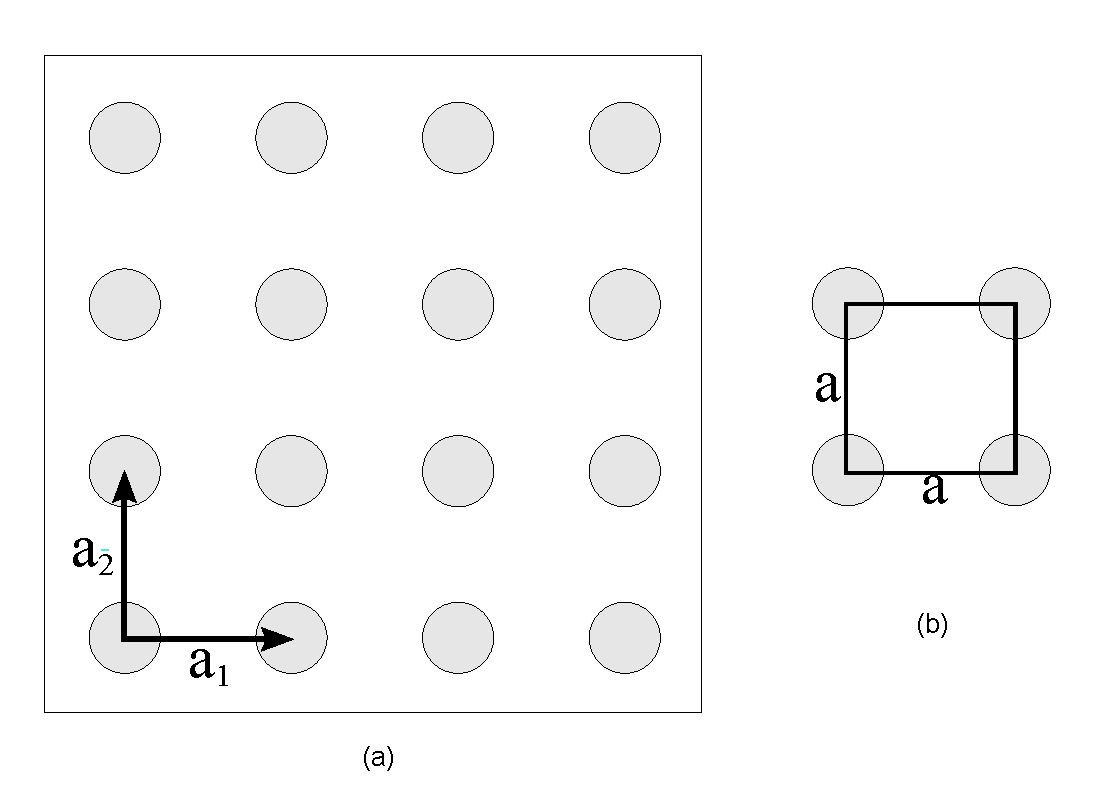
\includegraphics[scale=0.5]{./img/squarel.pdf}
\caption{Illustration of a bi dimensional point lattice: a) Section of a square lattice with primitive lattice vectors $a_1$ and $a_2$ b)  and one of the possible correspondent unitary cells where corners of four points are shared by one cell. Taken with permission from \cite{Guarin2012}.}
\label{fig:sq_lat_fig}
\end{figure}

So, if we have a 2D lattice of dielectric rods in air like in figure \ref{fig:sq_lat_fig} where the dielectric constant is a periodic function of space $\epsilon = \epsilon_0\epsilon_r(r)$\footnote{In which $\epsilon$ for air is $\epsilon(r) = \epsilon_0$ and inside the rod we have some positive realizable value $\epsilon_r$. And $r= x\hat{x}+y\hat{y}$}, then following what we learn in a solid state course we can define the crystal as a base (for example one rod) and a lattice. Which is the set of all discrete translation operations that are a linear combination of  multiples of the two primitive translation lattice vectors $a_1$ and $a_2$\cite{Kittel2005}. Or in a mathematical notation:
\begin{align}
&r' = r+u_1a_1+u_2a_2\\
& \hat{T}_{r'}\mathbf{E(r)} = \mathbf{R(r-r')} 
\label{eq:discrete_periodic}
\end{align}
where $u_1$ and $u_2$ are integers. If $\mathbf{E}$ is a plane wave, then we have 
\begin{align*}
\hat{T}_{r'}e^{i\vec{k}\cdot r} &= e^{i\vec{k}\cdot (r-r')}\\
\hat{T}_{r'}e^{i\vec{k}\cdot r} &= e^{i\vec{k}\cdot r} e^{i\vec{k}\cdot r'}
\end{align*}
with $\vec{k} = \vec{k}_x+\vec{k}_y$ as the wave vector with two components.
\begin{align}
\hat{T}_{r'}e^{i\vec{k}\cdot r} &= e^{i\vec{k}\cdot r} e^{i\vec{k}_x u_1a_1}e^{i\vec{k}_x u_2a_2}\label{eq:discrete_periodicity}
\end{align}

Now, \ref{eq:discrete_periodicity} does not immediately satisfy the form of equation \ref{eq:discrete_periodic} and we don't have an eigenfunction of the lattice. In order to get a solution that is invariant under discrete translations $r'$, the factor $e^{i\vec{k}\cdot r'}$ must be equal to 1, and this is obtained when one of two things happen, either $\vec{k}\cdot r' = 0$ or $\vec{k}\cdot r' = 2\pi n$ for $n = 1,2,3...$.
The first, is a trivial solution where there is no wave, on the other hand, the second is valid for any combination of $\vec{k_x}$ and $\vec{k_y}$ that happens to satisfy $\vec{k_x} = \frac{2\pi m}{a_1}$ and $\vec{k_y} = \frac{2\pi m}{a_2}$.  The minimal quantities $b_1 = \frac{2\pi}{a_1}$ and $b_2 = \frac{2\pi}{a_2}$ are known as the primitive vectors of the reciprocal lattice, and the linear combination of integer multiples of them form the reciprocal lattice (shown in figure ), which is the set of all arbitrary reciprocal lattice vectors defined by:

\[G = v_1b_1+v_2b_2\]

\begin{figure}
\centering
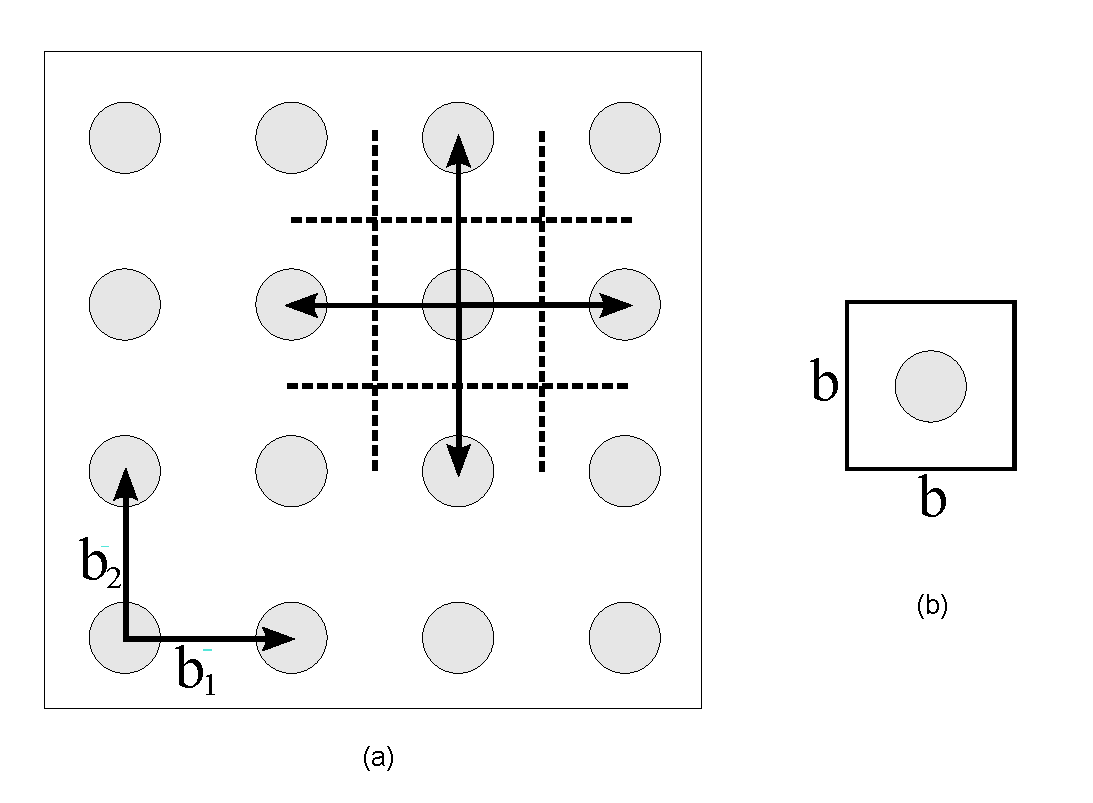
\includegraphics[scale=.5]{./img/squarer.pdf}
\caption{Illustration of a bi dimensional point lattice in the reciprocal domain: a) Section of a square lattice with primitive reciprocal lattice vectors $b_1$ and $b_2$ b)  and a reciprocal unitary cells best known as the first Brillouin zone. Taken with permission from \cite{Guarin2012}.}
\end{figure}

The nice thing about reciprocal lattice vectors is that a given wave vector $\vec{k}$ will have an indistinguishable effect on the wave from a wave vector $\vec{k} + G$ that is translated by a reciprocal lattice vector.  And remembering that $\hat{T_d}$ commutes with $\hat{\Theta}$, a general solution for $\mathbf{E}$ can be arranged by having a linear combination of the functions with different $\vec{k} + G$ that are solution to equation \ref{eq:discrete_periodic}. This is done as follows:

\begin{align*}
\mathbf{E(r)}_{\vec{k}} &= \sum_{m,n}C_{m,n}e^{i(\vec{k}+G_{m,n})\cdot r}\\
\mathbf{E(x,y)}_{k_x,k_y} &= \sum_{m,n}C_{m,n}e^{i(\vec{k}_x + mb_1)x}e^{i(\vec{k}_y + mb_2)y}\\
\mathbf{E(x,y)}_{k_x,k_y} &= e^{i\vec{k}_x x}e^{i\vec{k}_y y}\sum_{m,n}C_{m,n}e^{imb_1x}e^{imb_2y}\\
\mathbf{E(r)}_{\vec{k}} &= e^{i\vec{k}\cdot r} \mathbf{u}_{\vec{k}}(r)
\end{align*}

Where $\mathbf{u}_{\vec{k}}(r)$ is by definition a bi-periodic function in $r$ that satisfies  $\mathbf{u}_{\vec{k}}(r+r') = \mathbf{u}_{\vec{k}}(r)$ for a given $\vec{k}$.This result is commonly known as Bloch's Theorem, in solid state physics, and in mechanics as Floquet's. $C_{m,n}$ are expansion coefficients to be solved by explicit solution and are the key for the formulation of the Plane Wave Expansion (PWE) method \cite{Loaiza2011, Joannopoulos2008, StevenG.Johnson2001}. We however are not interested in $C_{m,n}$, because we are not solving for plane waves. Instead we will use this as a boundary condition by identifying how is the field after a translation of an arbitrary lattice vector $R$:

\begin{align}
\mathbf{E(r+R)}_{\vec{k}} &= e^{i\vec{k}\cdot (r+R)} \mathbf{u}_{\vec{k}}(r+R)\\
\mathbf{E(r+R)}_{\vec{k}} &= e^{i\vec{k}\cdot R}e^{i\vec{k}\cdot r} \mathbf{u}_{\vec{k}}(r)\\
\mathbf{E(r+R)}_{\vec{k}} &= e^{i\vec{k}\cdot R}\mathbf{E(r)}_{\vec{k}}
\end{align}

We now know that if $R$ is a lattice vector like $r'$, the solution of the field at that point will be exactly the same than the solution of the filed in the point before the translation multiplied by a complex factor $e^{i\vec{k}\cdot R}$. So given a known wave vector $\vec{k}$ and the solution of every point inside the base, or unitary cell, one can know the value of $\mathbf{E}$ everywhere. This is because the boundaries of a unit cell are separated by a distance that is either $a_1$ in $x$ or $a_2$ in $y$. Details about how to implement this condition in a numerical solution are given in \cite{Guarin2012}.

\subsection{Conservation of energy for waves in source less media}

We define the energy of a field $\mathbf{w}$ as its norm $||\mathbf{w}||^2 = \left(\mathbf{w},\mathbf{w}\right)$.
Conservation of energy in time in a source-less problem like that of equation \ref{eq:E-wave-loads} is obtained when $||\mathbf{w}||^2$ variation in time is zero, thus:
\begin{equation}
\frac{\partial ||\mathbf{w}||^2}{\partial t} =\frac{\partial \left(\mathbf{w},\mathbf{w}\right)}{\partial t} = \left(\dot{\mathbf{w}},\mathbf{w}\right)-\left(\mathbf{w},\dot{\mathbf{w}}\right) = \left(\hat{\Theta}\mathbf{w},\mathbf{w}\right)+\left(\mathbf{w},\hat{\Theta}\mathbf{w}\right) = \left(\hat{\Theta}\mathbf{w},\mathbf{w}\right)-\left(\hat{\Theta}\mathbf{w},\mathbf{w}\right) = 0
\end{equation}
Remembering that in a problem that is not harmonic we have $\hat{\Theta}\mathbf{E} = \frac{\partial^2 \mathbf{E}}{\partial t^2}$This means that under Hermitic operators such as $\hat{\Theta}$ the energy of the field is conserved\footnote{This expression for energy conservation holds only for cases where the operator does not change in time. A case where we have time varying material properties $\epsilon(r,t)$ can break conservation of energy if the time variation changes the norm\cite{Johnson07noteson}}.

\subsection{Energy functional of electromagnetic waves}
 
By means of the \textbf{electromagnetic variational theorem} we can formulate an energy functional to  to be minimized. This functional is defined as a normalized inner product between the function and the function multiplied by the following operator known as Rayleigh Quotient:
\begin{equation}
U_f(\mathbf{E}) \triangleq \frac{\left(\mathbf{E}, \hat{\Theta} \mathbf{E}\right)}{\left(\mathbf{E},\mathbf{E}\right)}
\label{eq:energy_functional}
\end{equation}

It is similar to other formulations used in fields like Quantum Mechanics and Classical mechanics such as expectation values, and energy Lagrangians.  The process of finding solutions that minimize such a potential is the core of what methods like Galerkin do for solving differential equations. In chapter \ref{ch:Finite_element_method} we will use a similar expression in order to solve the wave equation using Galerkin with Finite Elements.
 